%%%%%%%%%%%%%%%%%%%%%%%%%%%%%%%%%%%%%%%%%
% Journal Article
% LaTeX Template
% Version 1.3 (9/9/13)
%
% This template has been downloaded from:
% http://www.LaTeXTemplates.com
%
% Original author:
% Frits Wenneker (http://www.howtotex.com)
%
% License:
% CC BY-NC-SA 3.0 (http://creativecommons.org/licenses/by-nc-sa/3.0/)
%
%%%%%%%%%%%%%%%%%%%%%%%%%%%%%%%%%%%%%%%%%

%----------------------------------------------------------------------------------------
%	PACKAGES AND OTHER DOCUMENT CONFIGURATIONS
%----------------------------------------------------------------------------------------

\documentclass[twoside]{article}
\usepackage{datetime}
\usepackage{stackengine}
\usepackage{mathtools}
\renewcommand\useanchorwidth{T}
\usepackage{xcolor}
\def\theyearwidth{1.5pt}
\def\mystrut{\rule{0ex}{.1ex}}
\def\myyrstrut{\rule[-1ex]{0ex}{2ex}}
\newlength\yrsfboxrule
\yrsfboxrule .4\fboxrule
\newcommand\yearwidth[1]{\def\theyearwidth{#1}\ignorespaces}
\newcommand\skipyears[2][black]{%
  \fboxrule\yrsfboxrule%
  \fboxsep=-\yrsfboxrule%
  \fcolorbox{#1}{#1}{\mystrut\hspace{#2}}%
  \ignorespaces%
}
\newcommand\showyear[2][black]{%
  \fboxsep=0pt%
  \stackunder[2pt]{%
    \colorbox{#1}{\myyrstrut\hspace{\theyearwidth}}%
  }{\tiny#2}%
  \ignorespaces%
}
\usepackage{lipsum} % Package to generate dummy text throughout this template

\usepackage[sc]{mathpazo} % Use the Palatino font
\usepackage[T1]{fontenc} % Use 8-bit encoding that has 256 glyphs
\linespread{1.05} % Line spacing - Palatino needs more space between lines
\usepackage{microtype} % Slightly tweak font spacing for aesthetics

\usepackage[hmarginratio=1:1,top=32mm,columnsep=20pt]{geometry} % Document margins
\usepackage{multicol} % Used for the two-column layout of the document
\usepackage[hang, small,labelfont=bf,up,textfont=it,up]{caption} % Custom captions under/above floats in tables or figures
\usepackage{booktabs} % Horizontal rules in tables
\usepackage{float} % Required for tables and figures in the multi-column environment - they need to be placed in specific locations with the [H] (e.g. \begin{table}[H])
\usepackage{hyperref} % For hyperlinks in the PDF

\usepackage{lettrine} % The lettrine is the first enlarged letter at the beginning of the text
\usepackage{paralist} % Used for the compactitem environment which makes bullet points with less space between them

\usepackage{abstract} % Allows abstract customization
\renewcommand{\abstractnamefont}{\normalfont\bfseries} % Set the "Abstract" text to bold
\renewcommand{\abstracttextfont}{\normalfont\small\itshape} % Set the abstract itself to small italic text

\usepackage{titlesec} % Allows customization of titles
\renewcommand\thesection{\Roman{section}} % Roman numerals for the sections
\renewcommand\thesubsection{\Roman{subsection}} % Roman numerals for subsections
\titleformat{\section}[block]{\large\scshape\centering}{\thesection.}{1em}{} % Change the look of the section titles
\titleformat{\subsection}[block]{\large}{\thesubsection.}{1em}{} % Change the look of the section titles

\usepackage{fancyhdr} % Headers and footers
\pagestyle{fancy} % All pages have headers and footers
\fancyhead{} % Blank out the default header
\fancyfoot{} % Blank out the default footer
\fancyhead[C]{Approximation Algorithms for Stochastic Inventory Control Models $\bullet$ \ddmmyyyydate\today } % Custom header text
\fancyfoot[RO,LE]{\thepage} % Custom footer text

%----------------------------------------------------------------------------------------
%	TITLE SECTION
%----------------------------------------------------------------------------------------

\title{\vspace{-15mm}\fontsize{24pt}{10pt}\selectfont\textbf{Approximation Algorithms for Stochastic Inventory Control Models}} % Article title

\author{Hao Yuan
\and
Feng Wei
\and
Blake Miller
}
%----------------------------------------------------------------------------------------

\begin{document}

\maketitle % Insert title
\thispagestyle{fancy} % All pages have headers and footers

%----------------------------------------------------------------------------------------
%	ABSTRACT
%----------------------------------------------------------------------------------------

%\begin{abstract}%

%\noindent \lipsum[1] % Dummy abstract text%

%\end{abstract}
\begin{center}
{\ttfamily Github:\href{https://github.com/blakeapm/stochastic-inventory}{github.com/blakeapm/stochastic-inventory}}
\end{center}

%----------------------------------------------------------------------------------------
%	ARTICLE CONTENTS
%----------------------------------------------------------------------------------------

\begin{multicols}{2} % Two-column layout throughout the main article text

\section{Introduction}

\lettrine[nindent=0em,lines=2]{P}roper inventory management, stocking, and purchasing policy are paramount to supply, distribution, and retail businesses. The challenges of minimizing costs in an environment dependent upon many stochastic processes presents businesses with a unique challenge. This problem is important for any company that seeks to minimize cost of holding excess inventory while minimizing backorder costs (unmet demand). This is difficult because:
  \begin{compactitem}
    \item Oftentimes demand and lead times (time between order and receipt of product) are unpredictable.
    \item Inaccuracies can be extremely costly, so it is important that approximations are provably accurate within a certain range of error
  \end{compactitem}
It is also difficult to develop an approximation algorithm that is appropriate to the risk profile of companies operating under dynamic demand environments. This is because these companies must determine whether the provable error margin of an approximation algorithm is appropriate for their own risk profile. Computing a provably efficient inventory control policies is difficult because:
  \begin{compactitem}
    \item demand per time-period is correlated
    \item demand is non-stationary (time-dependent, distribution changes with time)
    \item cost is hard to predict due to the nature of demand
  \end{compactitem}
These algorithms are important in industries where the demand environment is highly dynamic. (i.e. Apple's supply-chain for solid state drives, seasonal products such as rock salt). These environments experience high correlation between demands in different periods (difficult to compute optimal inventory policy)

%------------------------------------------------

\section{The Model}
    We consider finite time horizon $T$:
    \par
      {\centering\yearwidth{1pt}\tclap{\tiny t}\showyear{1}\skipyears[black]{.25in}\showyear{2}\skipyears[black]{.25in}\showyear{3}\skipyears[black]{.25in}\showyear{4}\skipyears[black]{.25in}\showyear{5}\skipyears[black]{.25in}\showyear{6}\skipyears[black]{.25in}$\text{  }\cdots\text{  }$\showyear{$T-1$}\skipyears[black]{.25in}\showyear{$T$}
    \par}
    \vspace{0.1in}
    At each time period $t = 1,\cdots,T$, the following cost are incurred:
        \small
        \[L_t(x_t,d_t,q_t):=c_tq_t+h_t(x_t + q_t - d_t)^{+}+p_t(x_t + q_t -d_t)_{t}^{-}\]
        (Local Cost = Ordering Cost + Holding Cost + Backlogging Cost)
    The parameters represent the following:
    \begin{compactitem}
      \item $c_t$: per-unit ordering cost at time $t$.
      \item $h_t$: per-unit holding cost from $t$ to $t + 1$.
      \item $p_t$: per-unit backlogging penalty at time $t$.
      \item $x_t$: net inventory at time $t$. (our state)
      \item $q_t$: ordering quantity at time $t$. (our control)
      \item $d_t$: demand quantity at time $t$. (we observe $d_t$ after decide $q_t$)
    \end{compactitem}
    Our goal is to choose $q_t$ at time $t$ to minimize the expected total cost from period $t$ to $T$.\\
    To do this we will minimize the equations below. Let $V_t$ be the minimum expected cost from period $t$ to $T$. Then
    \begin{align}
    V_T(x_T,d_{1..T-1}) &= \min_{q_T \geq 0} E[L_T(x_T,D_T,q_T) | d_{1..T-1}] \nonumber\\
    V_t(x_t,d_{1..t-1}) &= \min_{q_t \geq 0} E[L_t(x_t,D_t,q_t)\nonumber\\
    & +V_{t+1}(x_t + q_t - D_t, d_{1..t-1},D_t)|d_{1..t-1}]\nonumber
    \end{align}
    This gives us two natural ways to "solve" the problem:
    \begin{compactitem}
      \item 
        Dynamic Programming: solve for $q_t$ backwards using the formula above.
      \item
        Myopic: At time $t$, ignore $V_{t+1}$, we only minimize $E[L_t(x_t,D_t,q_t)|d_{1..t-1}]$.
      \item 
        At period $s>t$, $D_s$ is a random variable that depends on perivous demands $d_1, d_2,...,d_{t+1},...,d_{s-1}$.\\
        To compute the above conditional expectation, we need to work on $q_t,...,q_T$ which are are our future decision.
      \item
        The myopic approach works extremely well on many cases\cite{CLAcha1}, but may perform extremely poorly on other cases. (We will explain a poorly-performing example at the end of the talk.)
    \end{compactitem}
    In fact we also need to consider leading time $L \neq 0$ (i.e. it takes $L$ periods to receive our order.) Then we need to modify:
        \begin{align}
          x_t & := Net~Inventory + Undelived~orders\nonumber\\
              & := Net~Inventory + \sum_{j = t - L+1}^{t-1} q_j\nonumber\\
          L_t(x_t,d_{t..t+L},q_t)& :=c_tq_t + h_{t+L}(x_t + q_t - \sum d_{t..t+L})^{+} \nonumber\\
                                &  + p_{t+L}(x_t + q_T - \sum d_{t..t+L})^{-}\nonumber
        \end{align}
        \[ \sum d_{t..t+L} := d_t + ... + d_{t+L}\]\\
        %***$Undelived~orders := \sum_{j = t - L+1}^{t-1} q_j$
    We can assume $c_t = 0$ by doing the transformation:
        \begin{align}
          \hat{c_t} &:= 0;\nonumber\\
          \hat{h_t} &:= h_t + c_t - c_{t+1}\nonumber\\
          \hat{p_t} &:= p_t - c_t + c_{t+1}\nonumber\\
          c_{T+1} &:= 0\nonumber
        \end{align}

    \textbf{Dual-Balancing Algorithm}\cite{CLAcha2}

    Recall {\em Local Backlogging Cost}:
    $$\Pi_t(x_t,q_t) := p_{t+L}(x_t + q_T - \sum D_{t..t+L})^{-}$$
    Now, we define {\em Marginal Holding Cost}:
    $$H_t(x_t,q_t) := \sum_{j = t+L}^{T} h_j (q_t - (\sum D_{t..j} - x_t)^+)^+$$.
    Dual-Balancing Algorithm:
    \begin{itemize}
      \item 
        Do transformation to make the ordering cost 0.
      \item
        Solve the convex optimization problem:
        $$q_t^* = argmin_{q_t > 0} \max{E[H_t(x_t,q_t)| d_{1..t-1}], E[\Pi_t(x_t,q_t)| d_{1..t-1}]}$$
        in order to find out $q_t^*$ such that
        $$E[H_t(x_t,q_t^*)| d_{1..t-1}] = E[\Pi_t(x_t,q_t^*)| d_{1..t-1}]$$
    \end{itemize}
\lipsum[4] % Dummy text

%------------------------------------------------

\section{Implementation}
\begin{center}
  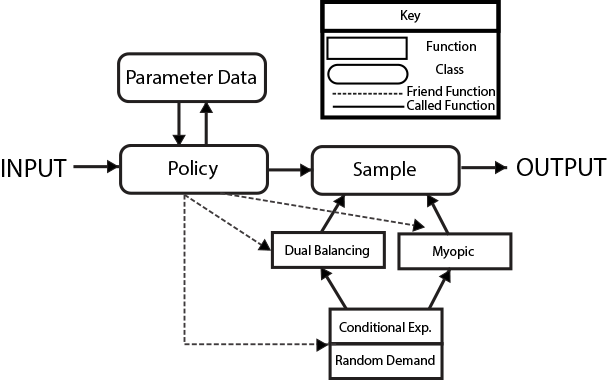
\includegraphics[width=3.0in]{software_diagram.png}
\end{center}

In following simulations:
    \begin{itemize}
      \item We always let $c_t = 3, h_t = 1, p_t = 2$.
      \item Without specific mention, time horizon $T = 100, L = 5, x_0 = 0$.
      \item The sample size is 20, if we do averages.
      \item We considered four different demands (i.e. $D_t$) distribution:\\
            1. $D_t = N(50,5)$ are iid.\\
            2. $D_t-D_{t-1} = N(5,1.581)$ with $D_0=30$.\\
            3. $D_t-D_{t-1} = B(10,0.5)$ with $D_0=30$.\\
            4. $D_t- (D_{t-1} + D_{t-2} + D_{t-3})/3 = N(5,1.581)$ with $D_0=30$.
    \end{itemize}

\section{Results}
  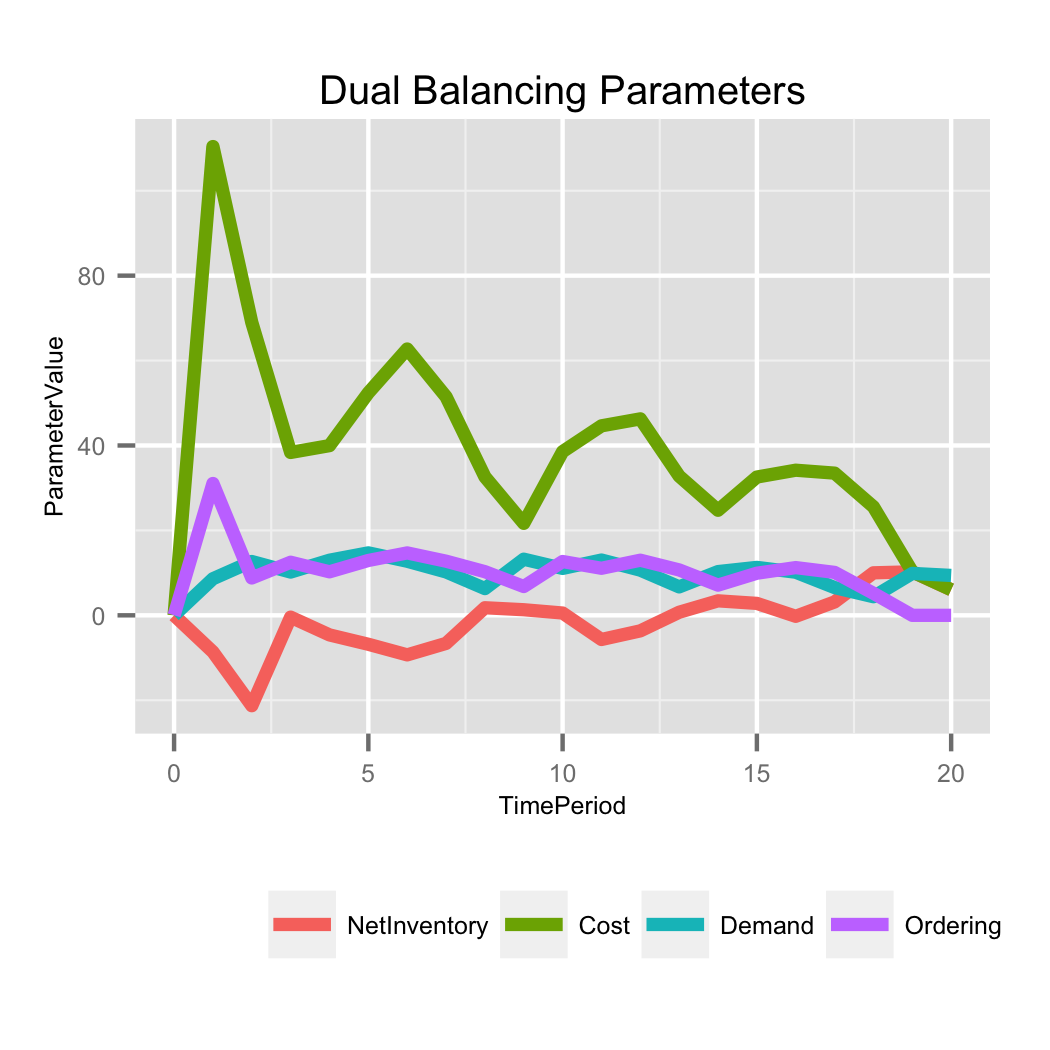
\includegraphics[width=3.0in]{figures/DualBalancingParameters.png}
  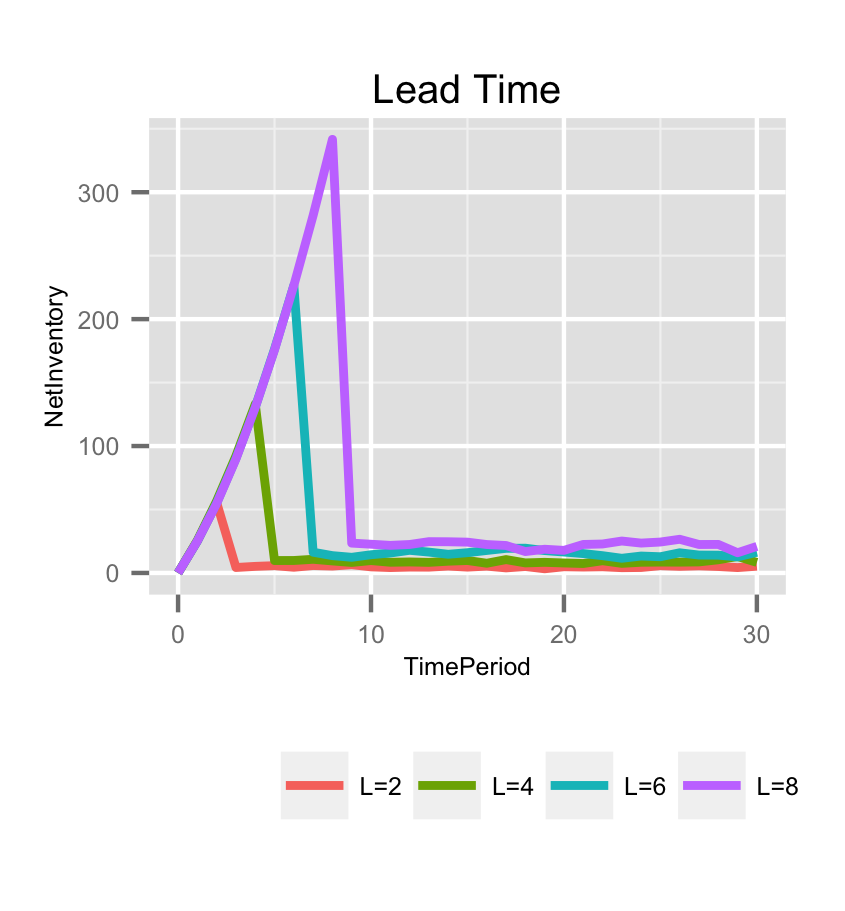
\includegraphics[width=3.0in]{figures/LeadTime.png}
  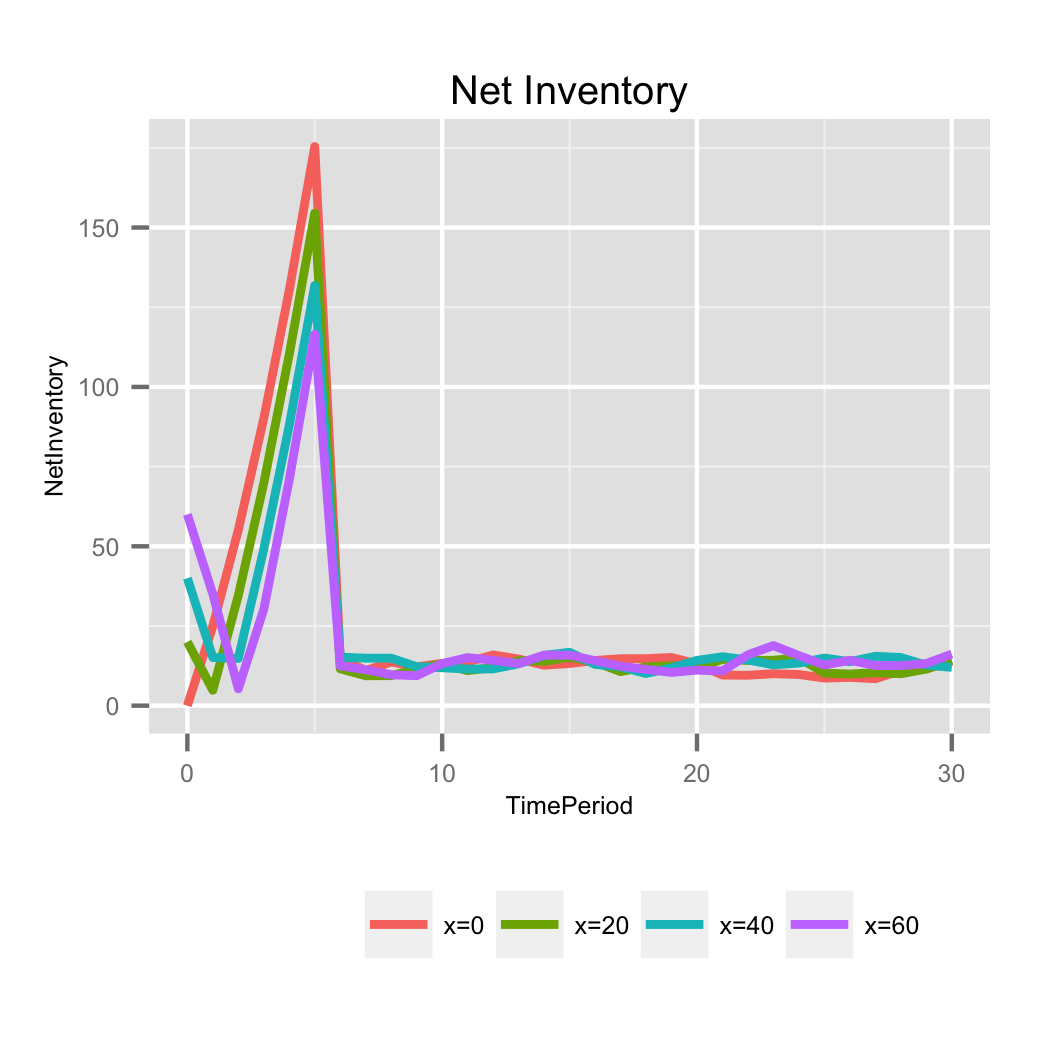
\includegraphics[width=3.0in]{figures/NetInventory.png}
  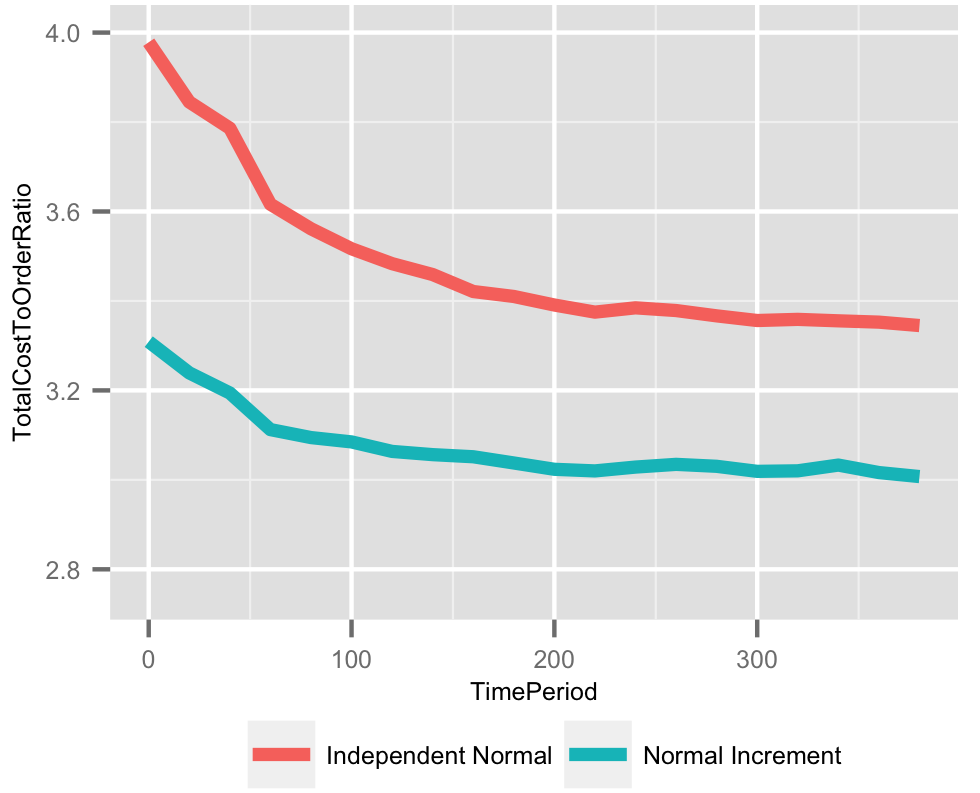
\includegraphics[width=3.0in]{figures/TotalCostToOrderRatio.png}
  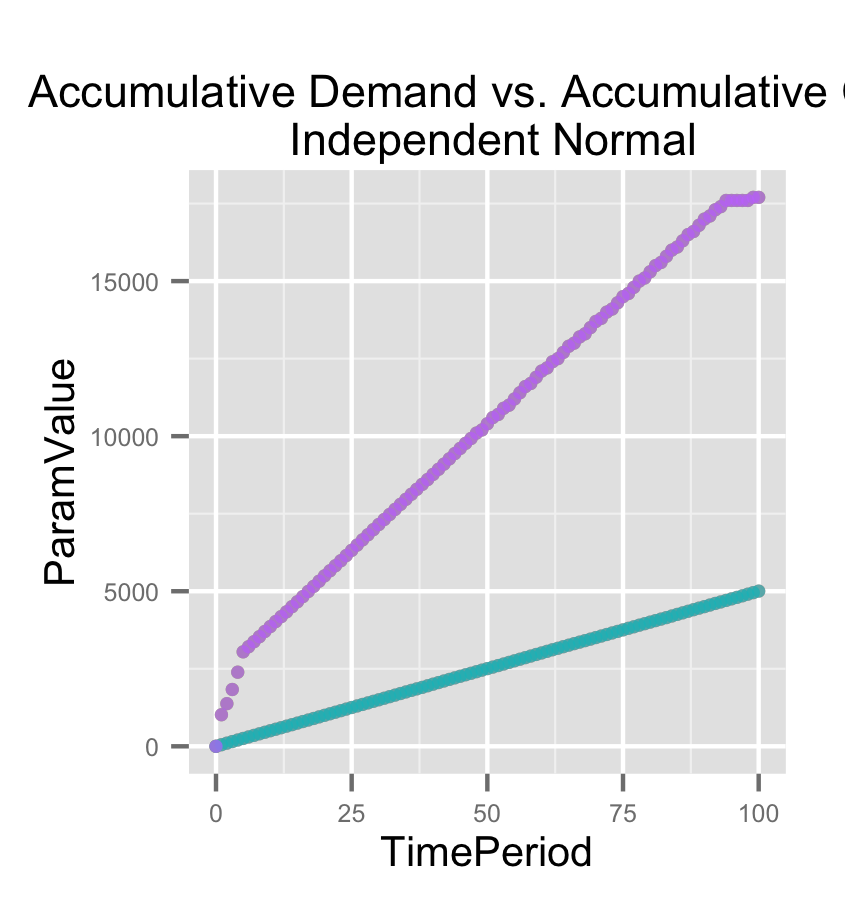
\includegraphics[width=3.0in]{figures/AccumulativeDemandAndCost_Normal.png}
  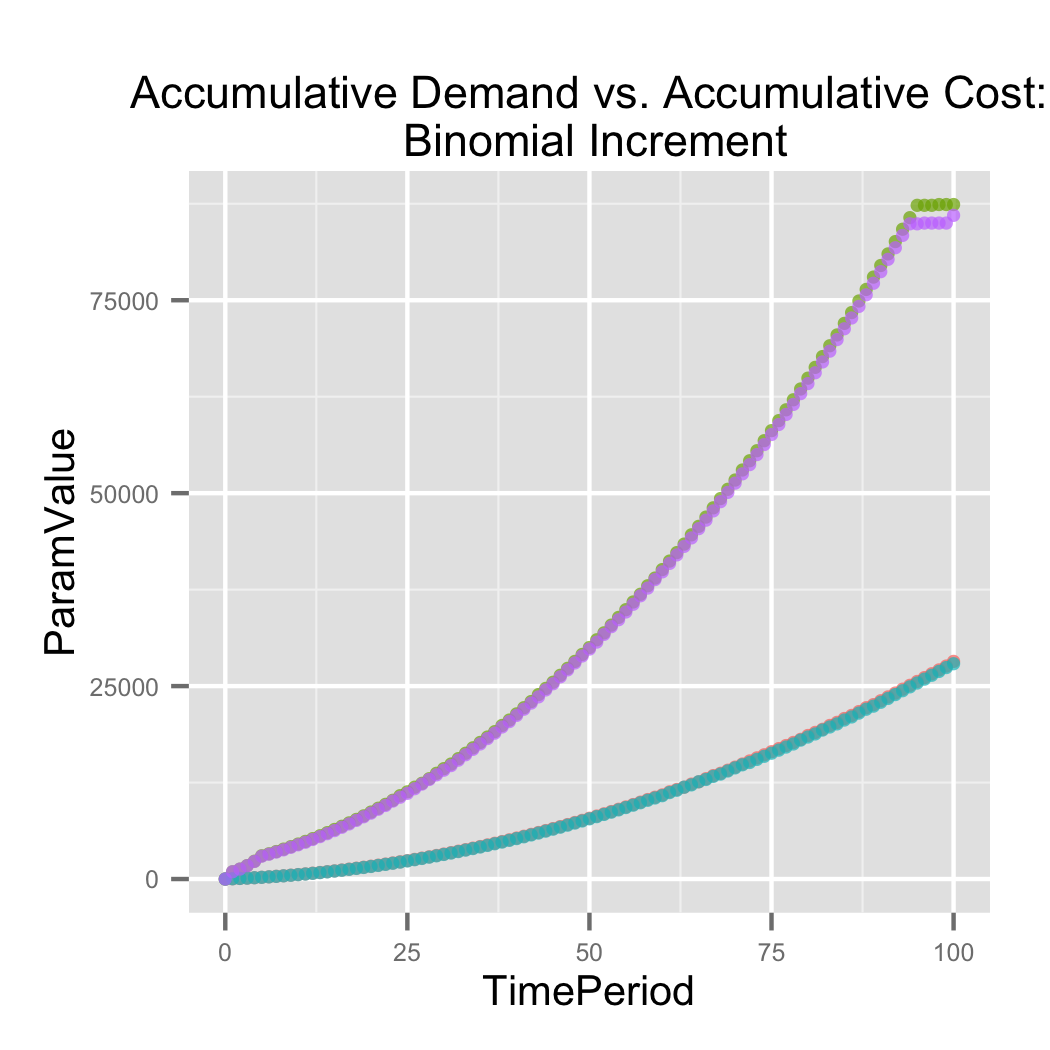
\includegraphics[width=3.0in]{figures/AccumulativeDemandAndCost_Binomial.png}
  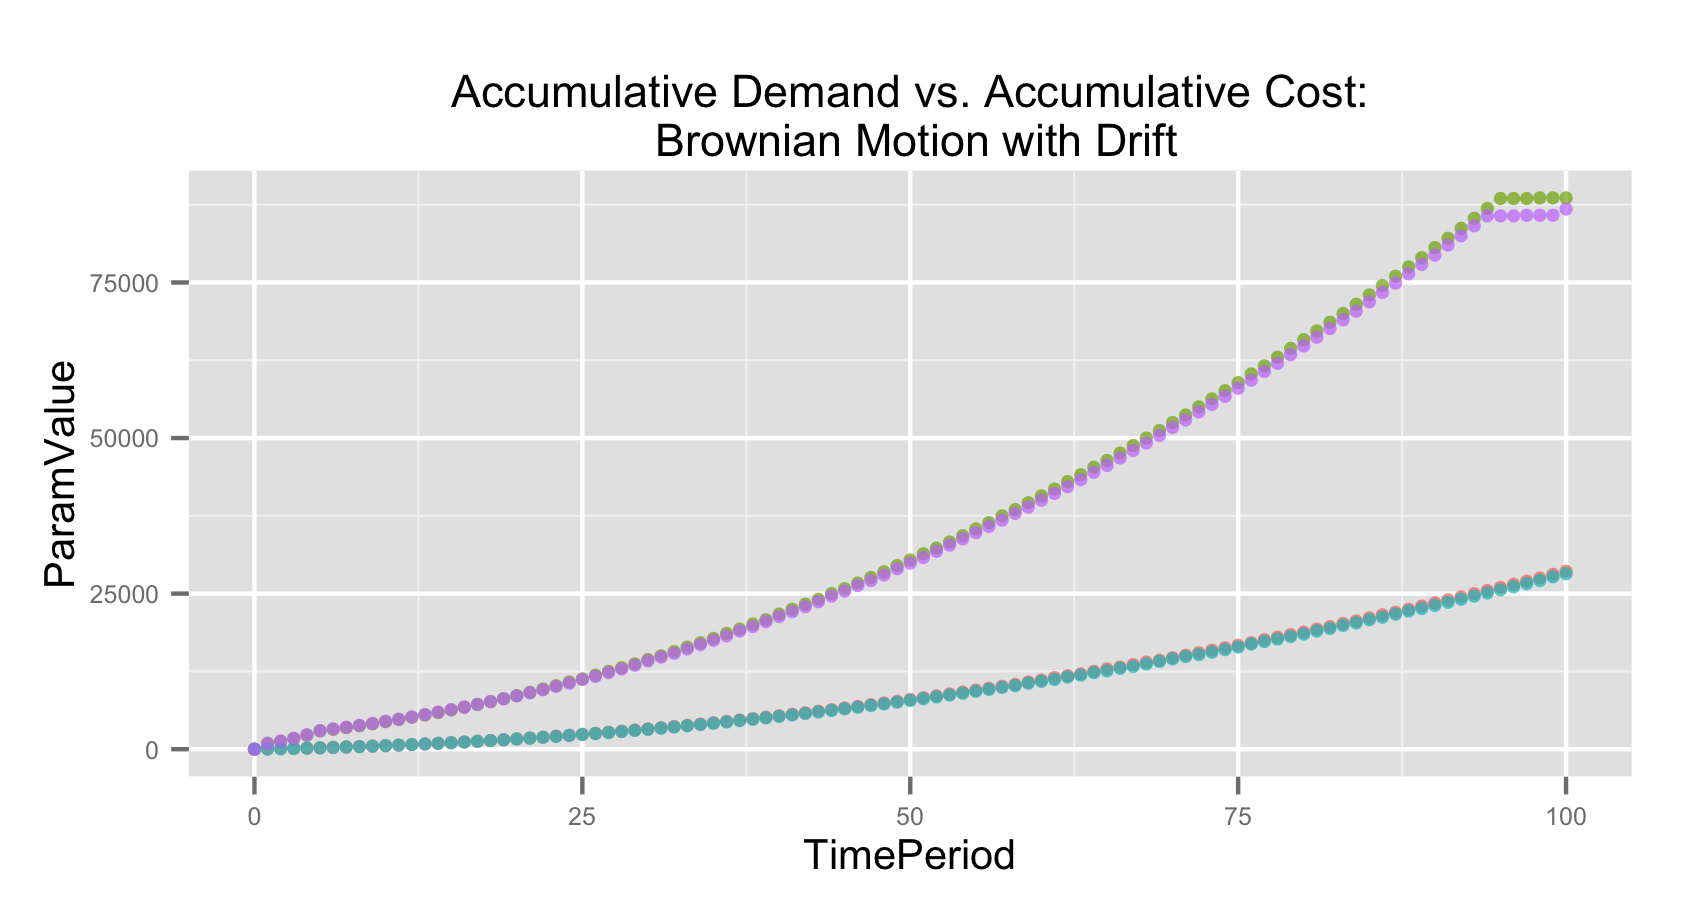
\includegraphics[width=3.0in]{figures/AccumulativeDemandAndCost_Brownian.png}
  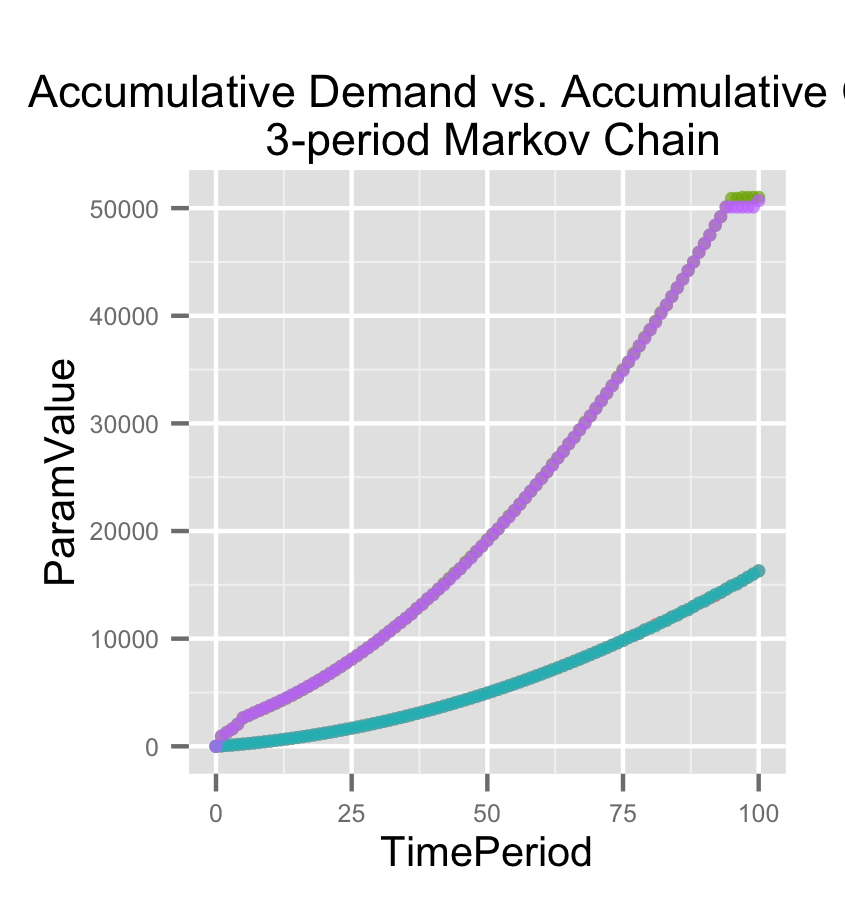
\includegraphics[width=3.0in]{figures/AccumulativeDemandAndCost_Markov.png}
  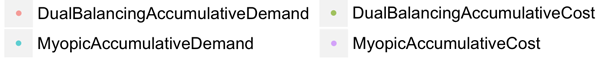
\includegraphics[width=3.0in]{figures/key.png}
  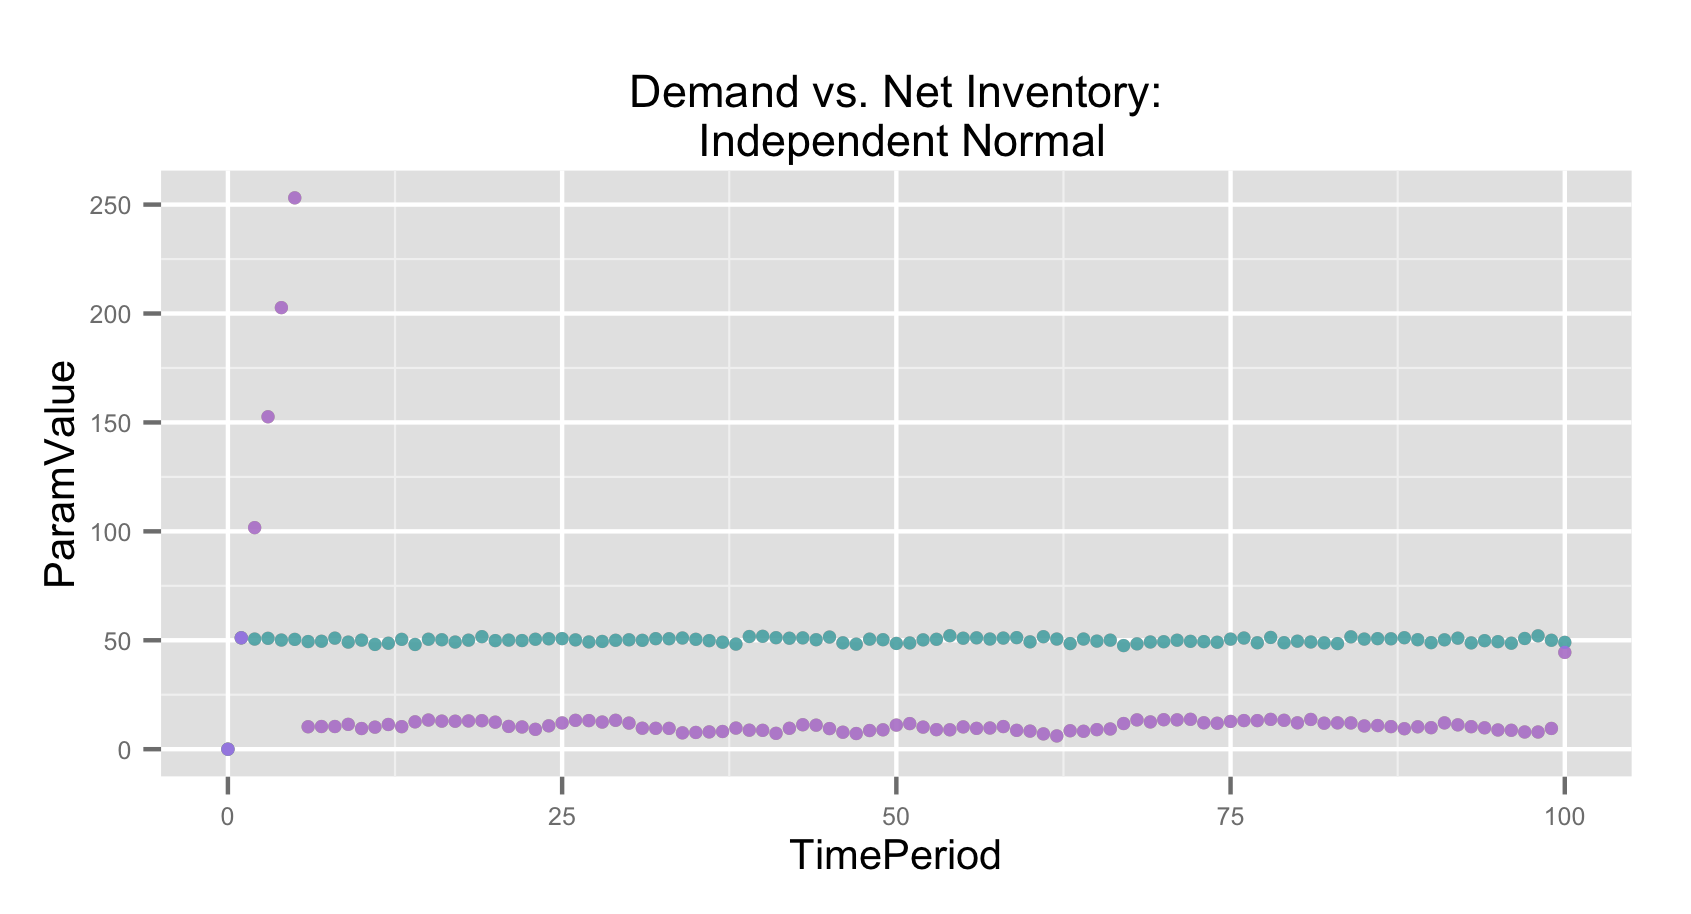
\includegraphics[width=3.0in]{figures/DemandAndNetInventory_Normal.png}
  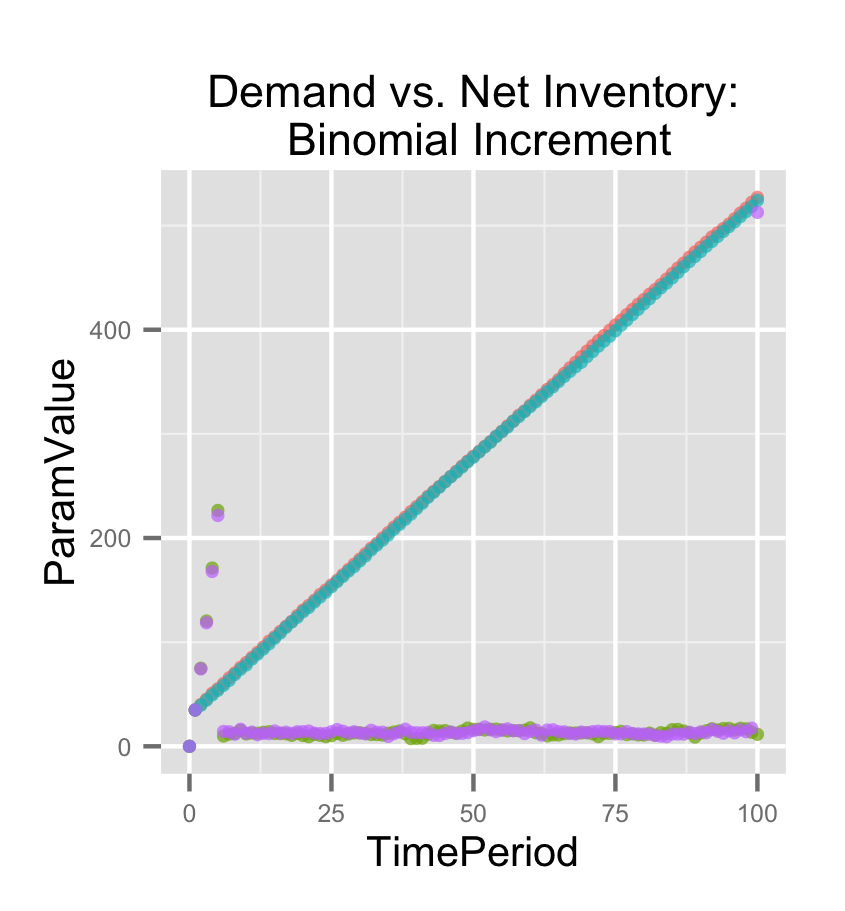
\includegraphics[width=3.0in]{figures/DemandAndNetInventory_Binomial.png}
  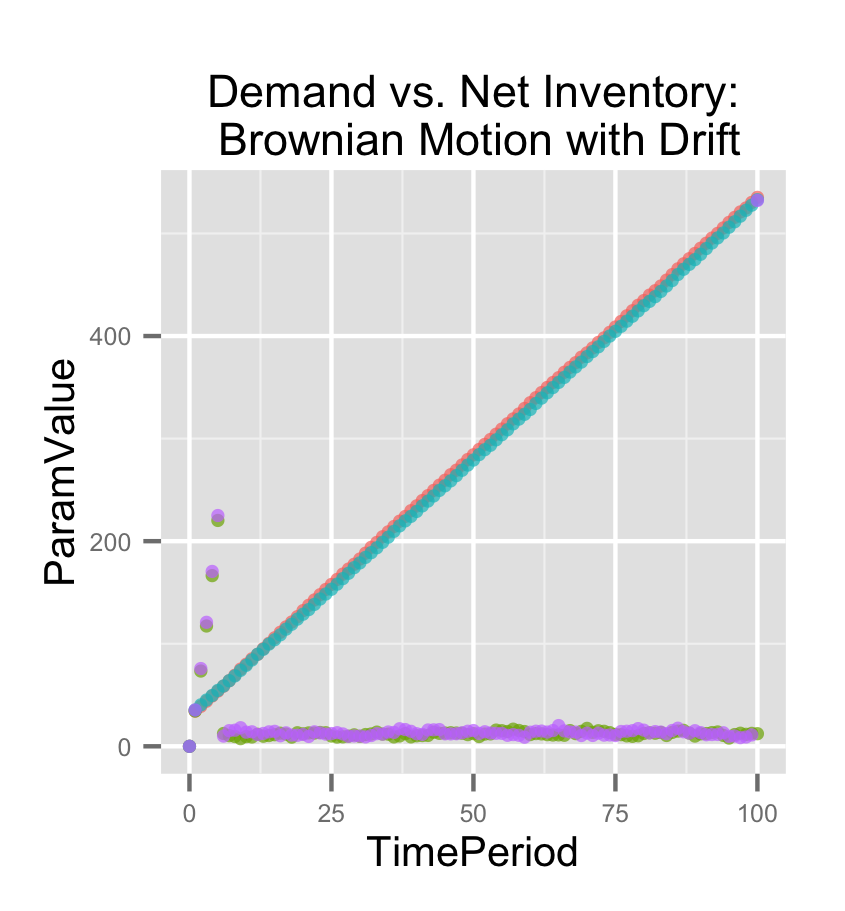
\includegraphics[width=3.0in]{figures/DemandAndNetInventory_Brownian.png}
  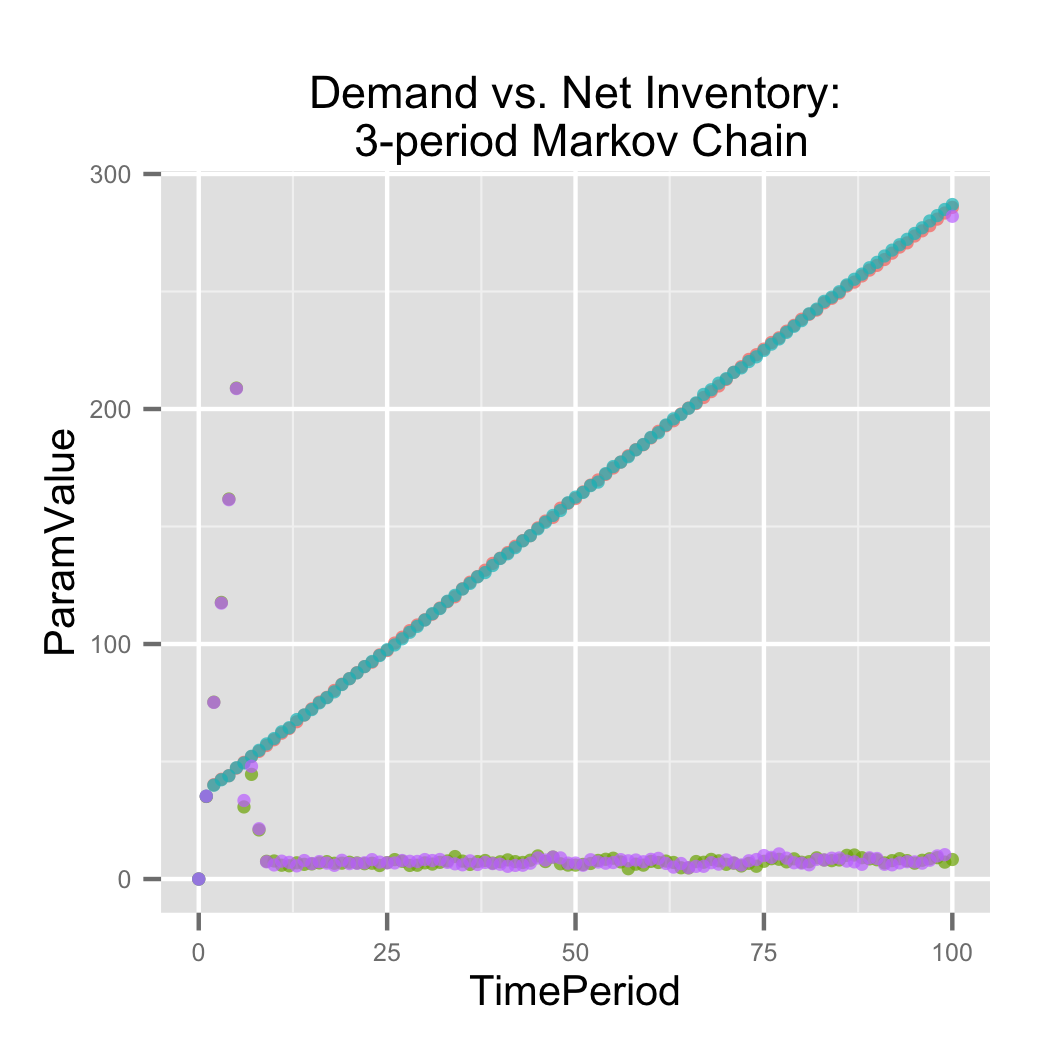
\includegraphics[width=3.0in]{figures/DemandAndNetInventory_Markov.png}
  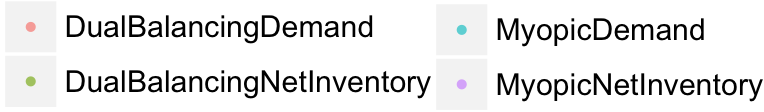
\includegraphics[width=3.05in]{figures/key2.png}
  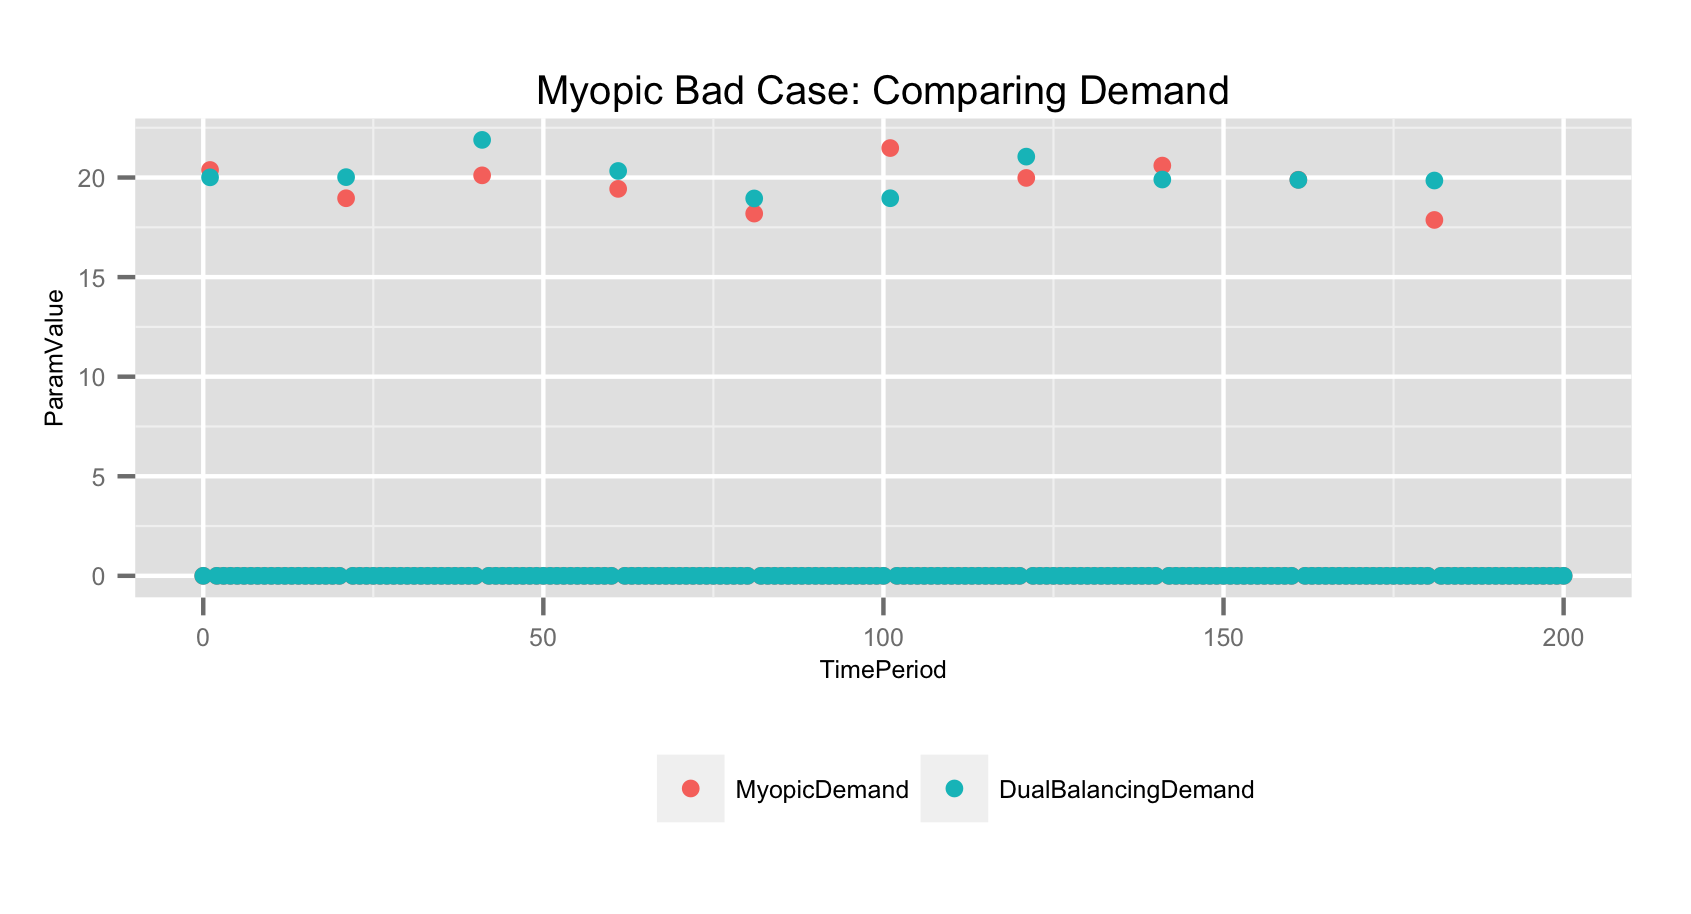
\includegraphics[width=3.0in]{figures/MyopicBadDemand.png}
  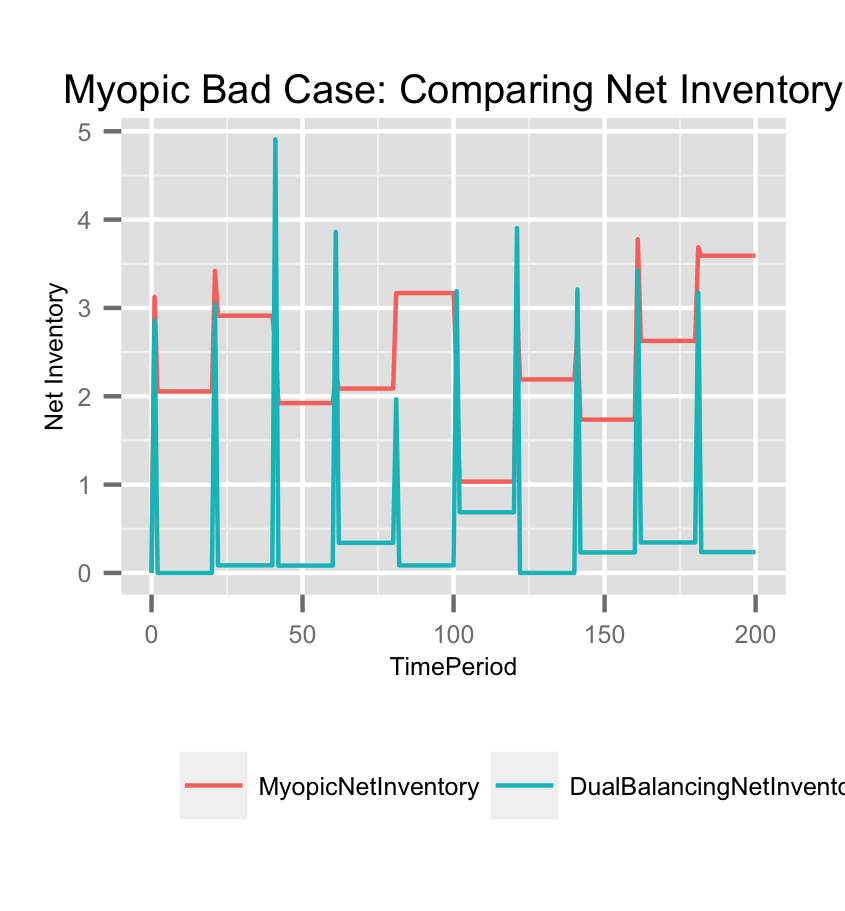
\includegraphics[width=3.0in]{figures/MyopicBadNetInventory.png}
  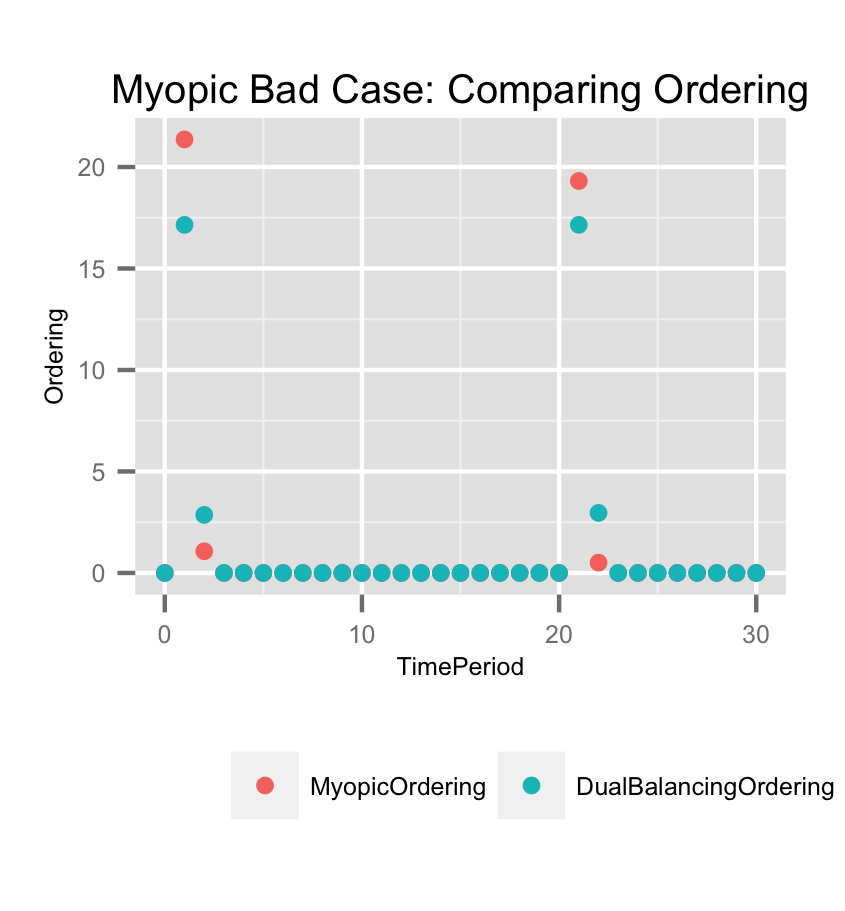
\includegraphics[width=3.0in]{figures/MyopicBadOrdering.png}
  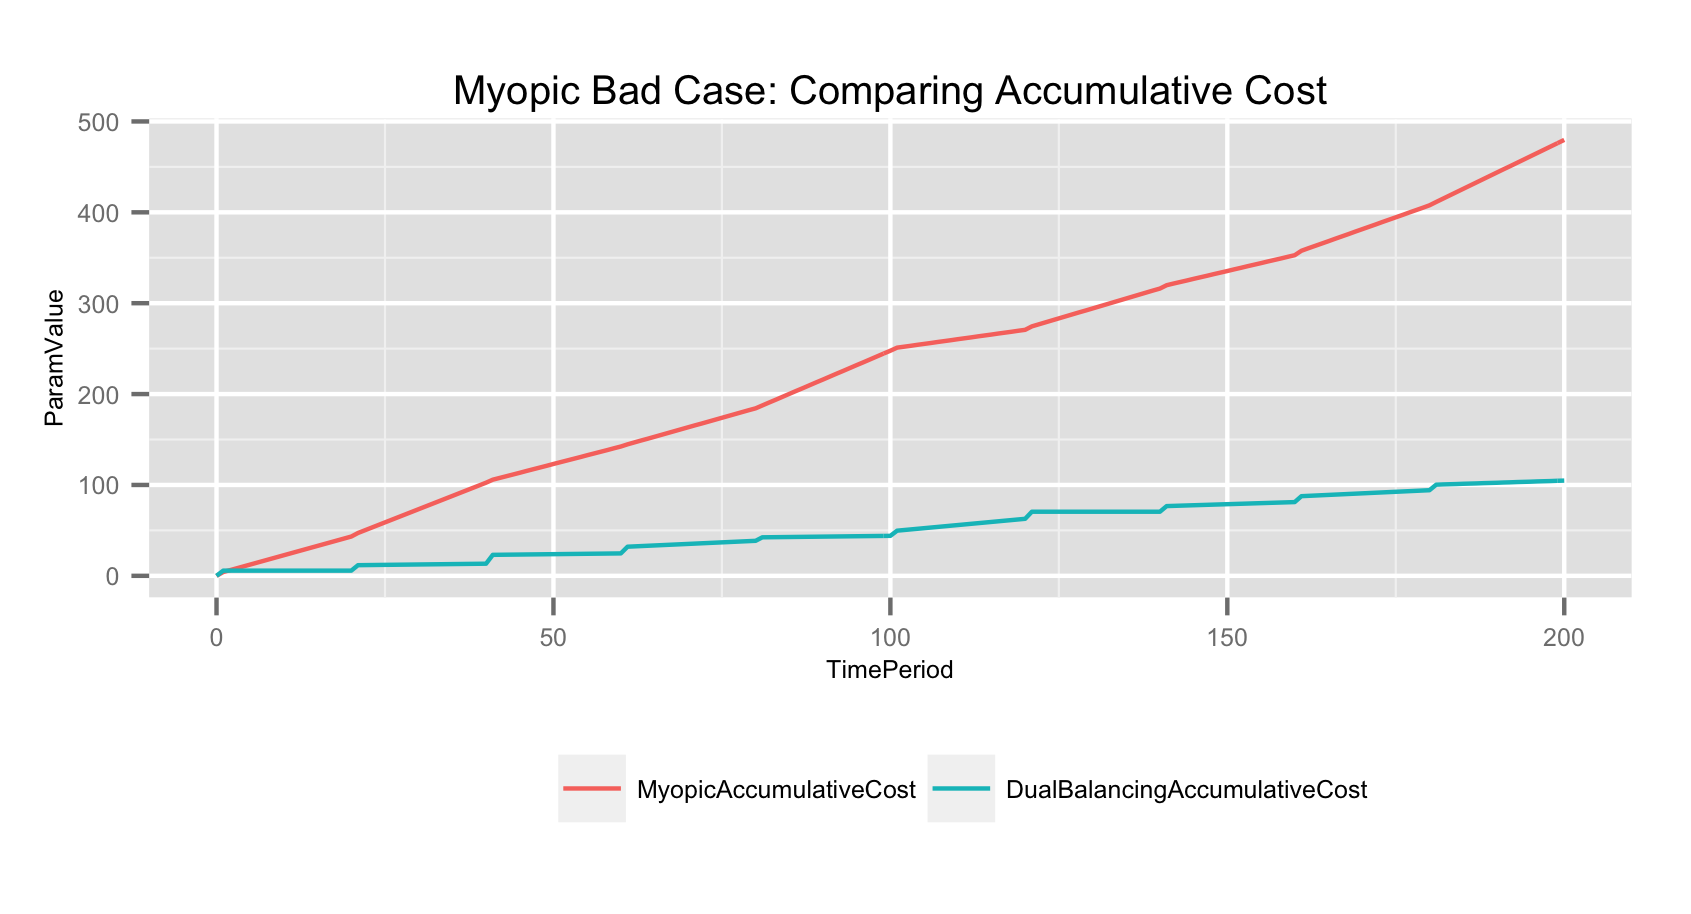
\includegraphics[width=3.0in]{figures/MyopicBadAccumulativeCost.png}
%------------------------------------------------

\section{Conclusion}

\lipsum[7] % Dummy text

%----------------------------------------------------------------------------------------
%	REFERENCE LIST
%----------------------------------------------------------------------------------------

\begin{thebibliography}{99} % Bibliography - this is intentionally simple in this template

\bibitem{CLAcha1}
Iida, T., P. H. Zipkin. 2006. Approximate solutions of a dynamic forecast-inventory model. Manufacturing Service Oper. Management
8 407-425.
\bibitem{CLAcha2}
Retsef Levi, Martin Pal, Robin Roundy and David Shmoys, 2007. Approximation Algorithms for Stochastic Inventory Control Models, Mathematics of Operations Research, Volume 32 (2), pages 284-302.

\end{thebibliography}

%----------------------------------------------------------------------------------------

\end{multicols}

\end{document}
